\section{Method}

In this section we are going to describe the dataset, the performed
preprocessing as well as details on the used neural network models. The
training and prediction was implemented using the Tensorflow library, see
Ref.~\cite{Tensorflow15}.\footnote{The training and prediction scripts are
available at \url{https://github/bodokaiser/mrtoct-tensorflow}.}

\subsection{Dataset}

There are several \gls{mri} and \gls{ct} datasets available, for
instance, \gls{oasis}~\cite{OASIS} or \gls{adni}~\cite{ADNI}. Unfortunately
public datasets in which both modalities are obtainable for the same subject
are, to date, rare. To our knowledge only the \gls{rire} project~\cite{RIRE}
and the Cancer Imaging Archive~\cite{CIA} provide \gls{mri} and \gls{ct}
volumes for some subjects. For the present work we limited ourselves to the
data from the \gls{rire} project, as the volumetric data was available in the
same format.
\begin{table}[h]
  \centering
  \begin{tabular}{*{6}{c}}
    \toprule
    & \multicolumn{4}{c}{\acrshort{mri}}
		& \\
   	\cmidrule{2-5}
    \acrshort{ct} &
		\acrshort{pd} &
		\acrshort{t1} &
		\acrshort{t2} &
		\acrshort{mp} \acrshort{rage} &
		\acrshort{pet} \\
    \midrule
    \num{17} & \num{14} & \num{19} & \num{18} & \num{9} & \num{8} \\
             & \num{12} & \num{17} & \num{16} & \num{9} & \num{6} \\
    \bottomrule
  \end{tabular}
  \caption{Subject statistics with respect of the available imaging
    modalities of the \gls{rire} dataset. The second table only accounts for
    subjects with available \gls{ct} data.
  }\label{tab:rire}
\end{table}
In \Cref{tab:rire} we list the aggregated modality count of the \gls{rire}
dataset (first row). As we use the \gls{ct} as target space, we created a
second modality count on the subjects with \gls{ct} modality (second row).
Beside of \gls{ct} one can also obtain \gls{pet} images for some subjects.
Next to the common \gls{t1} and \gls{t2} weighted \gls{mri}, some subjects of
the \gls{rire} dataset also offer \gls{pd} and \gls{mp} \gls{rage} weighted
\gls{mri}s. Some \gls{mri}s can be obtained in a rectified version, which we
did not use. We used the \gls{t1} weighted \gls{mri} together with the
\gls{ct} as input and target data as these give us the highest subject count.
However, it would be an interesting experiment to supply different \gls{mri}s
as multi-channel input.

\subsection{Preprocessing}

The modality data for each subject can be downloaded from the website of the
\gls{rire} project, see Ref.~\cite{RIRE}. In \Cref{fig:conversion} we depicted
the first preprocessing step, that involves the extraction, decompression and
conversion of the downloaded data. After extraction and decompression the
volumetric data presents itself as \gls{mhd}. We converted the \gls{mhd} files
to the self-contained \gls{nifti} format through the Python front-end of the
\gls{itk} library.
\begin{figure}[h]
  \centering
  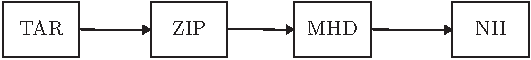
\includegraphics[page=1,width=.8\linewidth]{figure/diagrams.pdf}
  \caption{Image extraction and conversion from \gls{mhd} to \gls{nifti}
		format.
	}\label{fig:conversion}
\end{figure}
\Cref{fig:registration} illustrates the coregistration procedure as part of
the image preprocessing. The coregistration yields a rigid transformation that
aligns the moving volume with the fixed volume. In our case it makes sense to
use the \gls{ct} volume as the fixed volume because the \gls{ct} are in
general better centered. Given a rigid transformation, a linear interpolator
returns a translated volume from the sample points of the initial \gls{mri}.
The mutual information between the moved \gls{mri} and the \gls{ct} is then
used to optimize the rigid transformation. The procedure is executed
iteratively and stopped when the maximum iterations steps are reached or
the convergence parameter is met. As the implementation of the interpolator
and transformation optimizer is not a trivial undergoing, therefore we
reverted back to the \gls{itk} library, see Ref.~\cite{Yaniv2018}.
\begin{figure}[h]
  \centering
  \includegraphics[page=2,width=.8\linewidth]{figure/diagrams.pdf}
  \caption{Multi-modal image coregistration using maximum mutual information
    optimizer.
	}\label{fig:registration}
\end{figure}
Following the coregistration, we used the binary fill holes algorithm from
SciPy~\cite{SciPy} to remove the \gls{ct} table present in some \gls{ct}
volumes as well as well as background noise.\footnote{The complete
preprocessing described so far is available at
\url{https://github/bodokaiser/mrtoct-scripts}.} Finally we converted the
preprocessed pairs of \gls{mri} and \gls{ct} volumes to the tfrecord format
in order to easily read the data into Tensorflow~\cite{Tensorflow15}. As part
of the data pipeline implemented with Tensorflow we do a pad or crop to either
$384\times384$ for transverse 2D slices or $32\times32\times32$ for \gls{mri}
respective $16\times16\times16$ for \gls{ct} for 3D patches. The target shape
for the 2D slices was choosen to be compatible with the convolution parameters
and the largest resolution of all volumes. Furtheremore we applied a
min-max-normalization in order to operate on a value range of $[0,1]$.

\subsection{Models}

We implemented three different neural network models for the \gls{mri} to
\gls{ct} synthesis task. The first and most simple model is based on the
u-net model~\cite{Ronneberger15} and uses standard metric error metric,
i.e.\ \gls{mae} and \gls{mse}. The second model is based on
pix2pix~\cite{Isola16}, which already has proven great success in the task
of image translation. It uses the first u-net based model as generator in
addition to a discriminator model to calculate the adversarial loss. As third
model we implemented the context-aware 3D synthesis GAN from Nie~\cite{Nie16}.
In comparison to the other two models, which operate on the transverse 2D
slices of the brain, it is applied to 3D patches.

\subsubsection{u-net}

The original u-net model~\cite{Ronneberger15} was developed for the
segmentation of biomedical images. The key idea of the architecture is to
combine the capture of context and precise localization through interconnected
layers.
\begin{figure}[h]
  \centering
  \includegraphics[page=3,width=.8\linewidth]{figure/diagrams.pdf}
  \caption{The u-net generator architecture.
  }\label{fig:unet:gen}
\end{figure}
In \Cref{fig:unet:gen} the u-net architecture is illustrated. The
input \gls{mri} slice is of shape $384\times384\times1$, wherein the last
dimension corresponds to the number of channels. In case one would like to
input different weighted \gls{mri}s, it would be possible to concat these into
the last dimension as long as they are properly coregistered.
We can see that there are two paths of data flow: for one the image is passed
through a seqeunce of encoders and decoders, then again data can flow from
one encoder stage directly to the symmetric decoder stage. The encoder decode
features with increasing coarse resolution, while the decoders synthesize the
target image from the previous stage and the feature map of same resolution.
In \Cref{fig:unet:blocks} we present the exact layer composition of the
encoder, decoder and final block of the u-net architecture. In comparison to
the original u-net we reduced the convolution layers per block to one and
replaced the max-pooling in the decoders with deconvolutions. Furthermore
we used Leaky ReLUs in the encoders. These changes are mainly inspired by the
u-net like generator used in pixtopix. The first encoder block uses no batch
normalization and dropout is only used in Decoder \num{4} and Decoder \num{5}
as noted in \Cref{fig:unet:gen}.
\begin{table}[h]
  \centering
  \begin{tabular}{lrrc}
    \toprule
    Type & Kernel & Strides & Output Shape \\
    \midrule
    Input & & & \num{384x384x1} \\ 
    Convolution & \num{4x4} & \num{2} & \num{192x192x64} \\
    Convolution & \num{4x4} & \num{2} & \num{96x96x128} \\
    Convolution & \num{4x4} & \num{2} & \num{48x48x256} \\
    Convolution & \num{4x4} & \num{2} & \num{24x24x512} \\
    Convolution & \num{4x4} & \num{2} & \num{12x12x512} \\
    Deconvolution & \num{4x4} & \num{2} & \num{24x24x512} \\
    Deconvolution & \num{4x4} & \num{2} & \num{48x48x512} \\
    Deconvolution & \num{4x4} & \num{2} & \num{96x96x256} \\
    Deconvolution & \num{4x4} & \num{2} & \num{192x192x128} \\
    Deconvolution & \num{4x4} & \num{2} & \num{384x384x64} \\
    Deconvolution & \num{3x3} & \num{1} & \num{384x384x1} \\
    Output & & & \num{384x384x1} \\ 
    \bottomrule
  \end{tabular}
  \caption{Network parameters used in the u-net.
  }\label{tab:unet:conv}
\end{table}
In \Cref{tab:unet:conv} the convolution parameters for the convolution and
deconvolution layers in the u-net blocks are shown. The kernel paremeter
specifies the size of the convolution kernel, the stride parameter describes
the spacing in between applied convolutions. The padding algorithm was chosen
to keep output and input size the same. Weight initialization was performed
according using Xavier, see Ref.~\cite{Xavier2010}.

\subsubsection{pixtopix}

The pixtopix model uses the previously described u-net as generator in
addition to a discriminator to supply an adversarial score, see
Ref.~\cite{Isola16}. It has proven great success as general purpose solution
for translation experiments with color images. Recently the pixtopix was
extended to support training on unpaired data~\cite{Zhu2017}. This approach
has also already been applied successfully to the task of \gls{mri} to
\gls{ct} translation~\cite{Wolterink17}.
\begin{figure}[h]
  \centering
  \includegraphics[page=4,width=.8\linewidth]{figure/diagrams.pdf}
  \caption{The pixtopix discriminator architecture.
	}\label{fig:pixtopix:disc}
\end{figure}
In \Cref{fig:pixtopix:disc} the discriminator architecture is depicted. It
first concats the input \gls{mri} with either the target \gls{ct} or the
output \gls{ct}, depending on if we want to calculate a real or fake score,
in the channel dimension. The image of shape $384\times384\times2$ is then
passed through five convolutional layer that finally output a score map of
shape $1\times24\times512$.
In \Cref{fig:pixtopix:blocks} we see that the convolutional blocks comprise
a convolutional layer and a Leaky ReLU non-linearity, wherein the final block
uses a Sigmoid activation instead of Leaky ReLUs.
\begin{table}[h]
  \centering
  \begin{tabular}{lrrc}
    \toprule
    Type & Kernel & Strides & Output Shape \\
    \midrule
    Input & & & \num{384x384x2} \\ 
    Convolution & \num{4x4} & \num{2} & \num{192x192x64} \\
    Convolution & \num{4x4} & \num{2} & \num{96x96x128} \\
    Convolution & \num{4x4} & \num{2} & \num{48x48x256} \\
    Convolution & \num{4x4} & \num{2} & \num{24x24x512} \\
    Convolution & \num{4x4} & \num{1} & \num{1x24x512} \\
    Output & & & \num{1x24x512} \\ 
    \bottomrule
  \end{tabular}
  \caption{Network parameters used in the pixtopix discriminator.
  }\label{tab:pixtopix:conv}
\end{table}
\Cref{tab:pixtopix:conv} shows the exact configuration of the convolutional
layers in the pixtopix discriminator blocks.

\subsubsection{Context-aware 3D synthesis}

The last model uses 3D patches of shape $32\times32\times32$ from the
\gls{mri} to synthesize \gls{ct} patches of shape $16\times16\times16$. By
using a larger volume for the input the network is able to perform
context-aware synthesis. Furthermore the patch-based data approach allows the
support of different sized brain volumes or even only specific subregions ---
as long as the voxel size correspond to the same world sizes --- which is
useful for practical applications. Unfortunately this approach puts a lot
complexity in the pre- and postprocessing, as we need to extract the patches
first from the volume and then need to recombine them at a later stage.
\begin{figure}[h]
  \centering
  \includegraphics[page=5,width=.8\linewidth]{figure/diagrams.pdf}
  \caption{The contxt-aware 3D synthesis generator architecture.
  }\label{fig:synthesis:gen}
\end{figure}
\begin{figure}[h]
  \centering
  \includegraphics[page=6,width=.8\linewidth]{figure/diagrams.pdf}
  \caption{The context-aware 3D synthesis discriminator architecture.
	}\label{fig:synthesis:disc}
\end{figure}
In \Cref{fig:synthesis:gen} and \Cref{fig:synthesis:disc} we illustrated the
generator and discriminator architecture of the context-aware 3D synthesis
model. The generator iteratively convolves the input \gls{mri} patch to the
target \gls{ct} patch. In comparison to the u-net based generators there
are no interconnected layers. The discriminator takes a similar approach and
reduces the output or target \gls{ct} patch to a score map of shape
$8\times8\times8\times1$. In comparison to pixtopix it does not consider the
input \gls{mri}.
In \Cref{fig:synthesis:blocks} we see the internal structure of the
convolution blocks in both the generator and the discriminator. In comparison
to pixtopix it uses normal ReLUs and max pooling over deconvolution.
\begin{table}[h]
  \centering
  \begin{tabular}{lrrc}
    \toprule
    Type & Kernel & Strides & Output Shape \\
    \midrule
    Input & & & \num{32x32x32x1} \\ 
    Convolution & \num{9x9x9} & \num{1} & \num{24x24x24x32} \\
    Convolution & \num{3x3x3} & \num{1} & \num{24x24x24x32} \\
    Convolution & \num{3x3x3} & \num{1} & \num{24x24x24x32} \\
    Convolution & \num{3x3x3} & \num{1} & \num{24x24x24x32} \\
    Convolution & \num{9x9x9} & \num{1} & \num{16x16x16x64} \\
    Convolution & \num{3x3x3} & \num{1} & \num{16x16x16x64} \\
    Convolution & \num{3x3x3} & \num{1} & \num{16x16x16x32} \\
    Convolution & \num{7x7x7} & \num{1} & \num{16x16x16x32} \\
    Convolution & \num{3x3x3} & \num{1} & \num{16x16x16x32} \\
    Convolution & \num{3x3x3} & \num{1} & \num{16x16x16x1} \\
    Output & & & \num{16x16x16x1} \\ 
    \bottomrule
  \end{tabular}
  \caption{Network parameters used in the context-aware 3D synthesis generator.
  }\label{tab:synthesis:gen}
\end{table}
\begin{table}[h]
  \centering
  \begin{tabular}{lrrc}
    \toprule
    Type & Kernel & Strides & Output Shape \\
    \midrule
    Input & & & \num{16x16x16x1} \\ 
    Convolution & \num{5x5x5} & \num{1} & \num{16x16x16x32} \\
    Max Pooling & \num{3x3x3} & \num{1} & \num{14x14x14x32} \\
    Convolution & \num{5x5x5} & \num{1} & \num{14x14x14x64} \\
    Max Pooling & \num{3x3x3} & \num{1} & \num{12x12x12x64} \\
    Convolution & \num{5x5x5} & \num{1} & \num{12x12x12x128} \\
    Max Pooling & \num{3x3x3} & \num{1} & \num{10x10x10x128} \\
    Dense & \num{512} & & \num{8x8x8x512} \\
    Dense & \num{128} & & \num{8x8x8x128} \\
    Dense & \num{1} & & \num{8x8x8x1} \\
    Output & & & \num{8x8x8x1} \\ 
    \bottomrule
  \end{tabular}
  \caption{Network parameters used in the context-aware 3D synthesis
    discriminator.
  }\label{tab:synthesis:disc}
\end{table}
\Cref{tab:synthesis:blocks} discloses the convolution parameters used. Though
the kernel size was given in Ref.~\cite{Nie16}, we had to experiment with
the padding and the stride parameter in order to get the dimension reduction
to $16\times16\times\16$.
\begin{figure}[h]
  \centering
  \includegraphics[page=7,width=.8\linewidth]{figure/diagrams.pdf}
  \caption{The auto-context model used in ontext-aware 3D synthesis for
    image refinement.
	}\label{fig:synthesis:refine}
\end{figure}
We already noted that the context-aware 3D synthesis generator lacks
interconnected layers in comparison to u-net. Instead, it uses the
auto-context model first introduced in Ref.~\cite{Tu2010}. The concept is
illustrated in \Cref{fig:synthesis:refine}. The idea is to iteratively train
networks and to pass the previous results with the initial \gls{mri} to the
preceeding stage.
